\newpage
\pagenumbering{gobble} % Keine Seitenzahlen mehr

%-----------------------------------
% Ehrenwörtliche Erklärung
%-----------------------------------
\section*{Eigenständigkeitserklärung}

\noindent Hiermit versichere ich, dass ich die angemeldete Prüfungsleistung in allen Teilen eigen\-ständig ohne Hilfe von Dritten anfertigen und keine anderen als die in der Prüfungsleis\-tung angegebenen Quellen und zugelassenen Hilfsmittel verwenden werde. Sämtliche wörtlichen und sinngemäßen Übernahmen inklusive KI-generierter Inhalte werde ich kenntlich machen. Diese Prüfungsleistung hat zum Zeitpunkt der Abgabe weder in glei\-cher noch in ähnlicher Form, auch nicht auszugsweise, bereits einer Prüfungsbehörde zur Prüfung vorgelegen; hiervon ausgenommen sind Prüfungsleistungen, für die in der Mo\-dulbeschreibung ausdrücklich andere Regelungen festgelegt sind. Mir ist bekannt, dass die Zuwiderhandlung gegen den Inhalt dieser Erklärung einen Täuschungsversuch dar\-stellt, der das Nichtbestehen der Prüfung zur Folge hat und daneben strafrechtlich gem. § 156 StGB verfolgt werden kann. Darüber hinaus ist mir bekannt, dass ich bei schwerwie\-gender Täuschung exmatrikuliert und mit einer Geldbuße bis zu 50.000 EUR nach der für mich gültigen Rahmenprüfungsordnung belegt werden kann. Ich erkläre mich damit ein\-verstanden, dass diese Prüfungsleistung zwecks Plagiatsprüfung auf die Server externer Anbieter hochgeladen werden darf. Die Plagiatsprüfung stellt keine Zurverfügungstellung für die Öffentlichkeit dar.

\vspace{2cm}

\noindent\begin{tabular}{@{}p{0.5\textwidth}@{}p{0.5\textwidth}@{}}
{\raggedleft Bonn, 06.01.25} & {\raggedright\rule{5cm}{0.4pt}} \\
& {\raggedright Unterschrift}
\end{tabular}


% \par\medskip
% \par\medskip

\vspace{5cm}

% 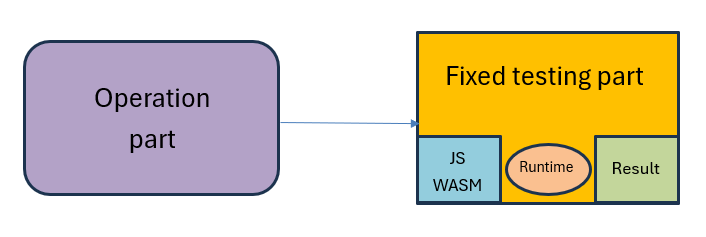
\includegraphics{signatures.png}